%%%%%%%%%%%%%%%%%%%%%%%%%%%%%%%%%%%%%%%%%
% Journal Article
% LaTeX Template
% Version 1.4 (15/5/16)
%
% This template has been downloaded from:
% http://www.LaTeXTemplates.com
%
% Original author:
% Frits Wenneker (http://www.howtotex.com) with extensive modifications by
% Vel (vel@LaTeXTemplates.com)
%
% License:
% CC BY-NC-SA 3.0 (http://creativecommons.org/licenses/by-nc-sa/3.0/)
%
%%%%%%%%%%%%%%%%%%%%%%%%%%%%%%%%%%%%%%%%%

%----------------------------------------------------------------------------------------
%	PACKAGES AND OTHER DOCUMENT CONFIGURATIONS
%----------------------------------------------------------------------------------------

\documentclass[twoside,twocolumn]{article}

\usepackage{blindtext} % Package to generate dummy text throughout this template 
\usepackage{graphicx}
\usepackage[sc]{mathpazo} % Use the Palatino font
\usepackage[T1]{fontenc} % Use 8-bit encoding that has 256 glyphs
\linespread{1.05} % Line spacing - Palatino needs more space between lines
\usepackage{microtype} % Slightly tweak font spacing for aesthetics

\usepackage[english]{babel} % Language hyphenation and typographical rules

\usepackage[hmarginratio=1:1,top=32mm,columnsep=20pt]{geometry} % Document margins
\usepackage[hang, small,labelfont=bf,up,textfont=it,up]{caption} % Custom captions under/above floats in tables or figures
\usepackage{booktabs} % Horizontal rules in tables
\usepackage{url}
\def\UrlBreaks{\do\/\do-}
\usepackage{lettrine} % The lettrine is the first enlarged letter at the beginning of the text

\usepackage{enumitem} % Customized lists
\setlist[itemize]{noitemsep} % Make itemize lists more compact

\usepackage{abstract} % Allows abstract customization
\renewcommand{\abstractnamefont}{\normalfont\bfseries} % Set the "Abstract" text to bold
\renewcommand{\abstracttextfont}{\normalfont\small\itshape} % Set the abstract itself to small italic text

\usepackage{titlesec} % Allows customization of titles
\renewcommand\thesection{\Roman{section}} % Roman numerals for the sections
\renewcommand\thesubsection{\roman{subsection}} % roman numerals for subsections
\titleformat{\section}[block]{\large\scshape\centering}{\thesection.}{1em}{} % Change the look of the section titles
\titleformat{\subsection}[block]{\large}{\thesubsection.}{1em}{} % Change the look of the section titles

\usepackage{fancyhdr} % Headers and footers
\pagestyle{fancy} % All pages have headers and footers
\fancyhead{} % Blank out the default header
\fancyfoot{} % Blank out the default footer
\fancyhead[C]{Effects of Banning Content on Online Hate Community Social Structure $\bullet$ February 2018} % Custom header text
\fancyfoot[RO,LE]{\thepage} % Custom footer text

\usepackage{titling} % Customizing the title section

\usepackage{hyperref} % For hyperlinks in the PDF

\usepackage{cite}

%----------------------------------------------------------------------------------------
%	TITLE SECTION
%----------------------------------------------------------------------------------------

\setlength{\droptitle}{-4\baselineskip} % Move the title up

\pretitle{\begin{center}\Huge\bfseries} % Article title formatting
\posttitle{\end{center}} % Article title closing formatting
\title{Effects of Banning Content on Online Hate Community Social Structure} % Article title
\author{%
\textsc{Vincent Wong, Yong-Yeol Ahn}\\[1ex] % Your name
\normalsize Indiana University \\ % Your institution
\normalsize \href{mailto:vmwong@indiana.edu}{vmwong@indiana.edu},  \href{mailto:yyahn@iu.edu}{yyahn@iu.edu} % Your email address
%\and % Uncomment if 2 authors are required, duplicate these 4 lines if more
%\textsc{Jane Smith}\thanks{Corresponding author} \\[1ex] % Second author's name
%\normalsize University of Utah \\ % Second author's institution
%\normalsize \href{mailto:jane@smith.com}{jane@smith.com} % Second author's email address
}
\date{\today} % Leave empty to omit a date
\renewcommand{\maketitlehookd}{%
\begin{abstract}
\noindent There has been increasing concern about the presence and moderation of hate content on social media. As these platforms ban hate groups, those communities exhibit backlashing. This raises the question about how banning these users affects the structure of the community they are in. To address this, I built and analyzed interaction networks from before and after the ban of the subreddit r/altright from Reddit, the discussion board platform. I find that the number of participants in this community decreases but the community structure doesn't appear to change. Despite this, the members of the communities appear to change greatly. This work contributes to understanding how administrative actions affect communities online. 
\end{abstract}
}

%----------------------------------------------------------------------------------------

\begin{document}

% Print the title
\maketitle

%----------------------------------------------------------------------------------------
%	ARTICLE CONTENTS
%----------------------------------------------------------------------------------------

\section{Introduction}

There is a common notion that the internet is renowned as a cesspool of hate \cite{wolchover}, but there are concerns about how the internet provides a platform that proliferates hate content in society at large \cite{manzar,sobkowicz,massanari}. Microblogging sites like Twitter \cite{twitterban}, discussion boards like Reddit \cite{redditban}, and VoIP applications like Discord \cite{discordban} have been removing users and communities deemed hateful. There are major discussions about the banning of hate speech.

This project studies how administrative removal of hateful communities impacts the social network of those communities. There are concerns about whether removing hateful content is effective at reducing the presence or accessibility of this content. In some cases, there is immediate backlash from these communities when their spaces for distributing content are removed, resulting in greater dissemination of the content in other spaces \cite{reddit2015details}. 

There is very little research about the effects of administrative action on social media, or about their effects on online social networks. Although a previous study found that the observed amount of hatespeech across Reddit decreased \cite{redditbanstudy}, it is not clear how the banning translated to the social dynamics that resulted in the backlash seen. 

To study this, I will look at the banning of a specific subforum of Reddit, the discussion board, as part of Reddit's attempts to crack down on hate content. I will use the subreddit 'altright' (stylized as 'r/altright'), a subreddit dedicated  to the alt-right movement, which was banned in early 2017 for allegedly breaking Reddit's terms of service regarding spreading personal information \cite{banaltright}. Banning r/altright was related to greater concerns about the increasing presence of far right groups in the American political climate around 2017. 

Using publically available historical Reddit post and comment data organized by subreddit, I built an interaction network from before and after the banning of r/altright to assess the impact this banning had on the social structure of reddit. By looking at the local social structure of users who posted on the banned subreddits, I can determine how user behaviors re-integrated or changed. A number of the community structures around r/altright stayed the same --- particularly the communities present in r/debatealtright (a closely related subreddit) and more general or popular reddits. Despite this, the actual members of these communities change significantly, and the total number of people in the community decreases. 

%OLD DISCUSSION: This research will uncover how the administrative policies of social media platforms affect their communities. It may inform methods to handle the moderation of this content in a way that ensures minimal subsequent damage and unintended consequence. Handling these issues requires understanding how the community structure will react in response to these major changes. Outside of the specific context of Reddit, there are broader concerns about how Internet communications may foster spaces for hate groups. The results of this project may inform how platforms’ actions affect the space of communities on the Internet as a whole. 

%------------------------------------------------

\section{Data}

Data was collected from the repository provided by Jason Baumgartner, also known by the username Stuck\textunderscore In\textunderscore the\textunderscore Matrix, who hosts full collections of Reddit data on his website, pushshift.io \cite{pushshift}. Although Reddit has an API for requesting data \cite{redditAPI}, the API would only allow pulling data that is publicly available now, which would exclude banned subreddits. Because the dataset from pushshift.io had started in response to the 2015 bannings of subreddits including r/FatPeopleHate and r/CoonTown, we were unable to use those subreddits for this case study as they were missing from pushshift.io. We chose r/altright for this case study because the data is available and the banning appears to have had a similar subreddit spinoff effect. 

Reddit does not provide information on the specific date or time that a subreddit is banned, opting for approximate time stamps truncated at the largest scale since the ban (r/altright was banned roughly "1 year ago" \cite{raltright}). We estimated the date of the ban by referencing a number of different news sources published at the tim of the ban \cite{banaltright} and concluded that the ban occurred on either January 30th or February 1st, 2017. 

Using this, we downloaded the reddit comment data for the preceeding and following two months around the ban. In our case, we downloaded comment data from December 2016 and January 2017 before the ban, and February 2017 and March 2017 after it. 

To constrain the population of users of interest, we gather a list of all the users who had commented in r/altright in January 2017, the month before the ban. We are primarily interested in seeing if their interactions changed greatly due to the ban, so we gather all of the comments made by these users within our four month dataset. This comprises our content of interest. 

%------------------------------------------------

\section{Methods and Results}

\subsection{Constructing Networks}

In order to understand the affect of the ban on the community structure, we create networks of interactions between users before and after the ban. We then look at a number of metrics to characterize the differences between the networks between months. In particular, we are interested in the correspondence between membership in detected communities before and after the ban. A high correspondence would indicate that a sufficient number of users remain on Reddit and continue to interact in a manner similar to their interactions prior to the ban. A low correspondence would indicate that the communities changed drastically, either due to shuffling, removal, or replacement. 

Networks were constructed by creating an edge between two users if both users had participated in at least two threads together within the month in question. This resulted in four temporal networks, each one created for the month of data we gathered. Because users cannot interact in the subreddit after it is banned, we were primarily interested in the community structure around the subreddit. For this, we only considered comments in threads outside of the subreddit. The networks from the months before the ban are shown in Fig. \ref{fig:1}, and the networks from the months after the ban are shown in Fig. \ref{fig:2}.

%Figures

We provide some basic summary statistics in Table \ref{table1}. It is clear from the number of nodes in the networks that roughly 30\% of users who had commented in r/altright no longer met our criterion for appearing in the network (that is, they no longer commented on threads with any other user at least twice). 

%Table1

\subsection{Analyzing Networks}

We are interested in determining if the removal of the users due to the ban is significantly different than if the same number of users had left by random chance. To do this, we construct a null model for the network from February 2017 by taking the network from January 2017 and randomly deleting nodes until the network contained the same number of nodes as that of February 2017. We calculate a number of metrics to characterize this null model, and compare the same metrics for the real case against a distribution of 500 null model trials. 

To be able to compare the differences in communities from before and after the ban, we calculate the minimum Jaccard distance between the members of each of the communities. Communities were first determined using the Louvain method for community detection \cite{louvain}. Because many assignments could exist between communities over time, we want to get the minimum dissimilarity (maximum overlap) between communities when they are mapped to each other. To do this, we use the Hungarian method to address the assignment problem that minimizes the cost between communities \cite{dedecko}. We calculate the cost matrix for assigning one community from one network to another in another network, where each cost is one minus the Jaccard similarity. The Hungarian method provides the optimal mapping between communities, as well as the minimized potential due to the cost of creating the mapping, which is the Jaccard distance. We will refer to the minimized potential reported from the Hungarian method as the community overlay distance. 

The results of this test are shown in Table \ref{table2}. We find that, for many of the basic metrics that assess the micro-scale characteristics of the network (such as mean degree, which focuses entirely on the nodes), there is no significant difference between the two networks. The mean shortest path length ($p<0.01$) and assortativity ($p<0.01$) are higher than the null models. This may be due to the choice in null model, because it does not distinguish between communities that restructured due to the loss in users, or the loss in communities due to specific (non-random) loss of users. 

%Table2

We find that the community overlay distance is much, much higher than the null model would indicate. This means that the communities of the real network have a significantly different user composition compared to those of the null model. We can eliminate the possibility that the users are being cycled out with new users because we only look at the users who had posted in r/altright in January 2017 based on their interactions in the following month. This likely means that users are shifting their places in the communities of interaction. 

%average degree, network diameter, average shortest path length, assortativity, density, average clustering coefficient, number of cliques, transitivity (number of actual triangles over the number of possible triangles), and community overlay distance. 

\subsection{Characterizing Communities}

In order to get a better understanding of the participation of users in the networks we created, we characterized communities by the subreddits in which those users most often commented. To do this, we took the edges (user-user pairs) within the communities in a given network for a given month, and tracked the counts of subreddits where those comments occurred. This ensured that the counts of subreddits were still bounded by the conditions to create the graph, namely that the two users needed to comment in the same thread at least twice. 

When we did this, we found that the communities maintained subreddit identity over time. For the largest communities prior to the banning of r/altright, there was a highly connected group who primarily commented in r/debatealtright, the subreddit for discussion of alt-right issues from an alt-right perspective. There were also communities characterized by greater general use of Reddit (with some very common subreddits about topics about sports and computers, as well as r/AskReddit), and communities with this same popular bent but including r/The\textunderscore Donald, the subreddit dedicated to Donald Trump. 

Notably, in the networks prior to the banning of r/altright, there is a small and distant community that primarily participated in r/MGTOW (Men Going Their Own Way) and r/theredpill, both of which are subreddits nominally dedicated to the emotional support for men, but are dominated by sexist and anti-social-justice rhetoric. 

After the ban, these same communities persist, including the community around popular subreddits, and particularly the community around r/debatealtright. This is important because r/debatealtright is so similar to the topic of r/altright that it is surprising that it was not banned. This may be due to the very fine line that Reddit has tread when taking a stance against this kind of content \cite{banaltright}

Finally, it is important to note that no new communities appear in subreddits that attempt to circumvent the ban (such as r/altright2, r/altright3, etc). Although specific ban dates for all of these subreddits by any other name are not released, it at least appears that the community did not persist in a subsequent subreddit. 

\section{Conclusion}

In this project, we investigate the effects of banning the subreddit r/altright on Reddit on the community structure around that subreddit. By investigating the interaction networks of users from these subreddits before and after the ban, I determine the ban did not affect the general community structure in subreddits that shared user participation with r/altright. However, the total participation in the community decreased significantly, and the membership in these communities also changed greatly. 

In the future, I would like to investigate the alternative routes that users in those subreddits used to continue expressing their demand for the banned content. In particular, it may be possible to derive the appearance of subsequently spawned subreddits (such as r/altright2, r/altright3, etc) by looking at the subreddit location of posts created by users in the dataset. 

I would also want to look at the subreddit over a larger span of time to see how consistently the network maintains its population over time. This would also give the opportunity to investigate whether the communities change over a longer period of time. In context of understanding the effects of administrative action on online communities, this would be crucial to understanding whether there is long-term benefit to banning subreddits. 

%------------------------------------------------


%----------------------------------------------------------------------------------------
%	REFERENCE LIST
%----------------------------------------------------------------------------------------

\begin{thebibliography}{99} % Bibliography - this is intentionally simple in this template

\bibitem{wolchover} Wolchover, Natalie. "Why Is Everyone on the Internet So Angry?" Scientific American. July 15, 2012. Accessed February 2018. \url{https://www.scientificamerican.com/article/why-is-everyone-on-the-internet-so-angry/}
 
\bibitem{manzar} Manzar, Osama. "Hate speech and the role of social media." Livemint. February 9, 2018. Accessed February 12, 2018. \url{http://www.livemint.com/Opinion/ZAHBp4YDLp1BcCnlIuwFON/Hate-speech-and-the-role-of-social-media.html}
 
\bibitem{sobkowicz} Sobkowicz, P., Sobkowicz, A. "Dynamics of hate based Internet user networks." Eur. Phys. J. B (2010) 73: 633. https://doi.org/10.1140/epjb/e2010-00039-0

\bibitem{massanari} Massanari, Adrienne. "\# Gamergate and The Fappening: How Reddit’s algorithm, governance, and culture support toxic technocultures." New Media \& Society. Vol 19, Issue 3, pp. 329 - 346. https://doi.org/10.1177/1461444815608807

\bibitem{twitterban} Neidig, Harper. "Twitter launches hate speech crackdown." The Hill. December 18, 2017. Accessed February 2018. \url{http://thehill.com/policy/technology/365424-twitter-to-begin-enforcing-new-hate-speech-rules}

\bibitem{redditban} Robertson, Ali. "Reddit bans 'Fat People Hate' and other subreddits under new harassment rules". The Verge. June 10, 2015. Accessed February 2018. \url{https://www.theverge.com/2015/6/10/8761763/reddit-harassment-ban-fat-people-hate-subreddit}

\bibitem{discordban} Newton, Casey. "Discord bans servers that promote Nazi ideology." The Verge. August 14, 2017. Accessed February 2018. \url{https://www.theverge.com/2017/8/14/16145432/discord-nazi-ban-white-supremacist-altright}
  
\bibitem{reddit2015details} Koebler, Jason. "This Is the Site Redditors Are Migrating to Now That r/FatPeopleHate Is Banned". VICE: Motherboard. June 10, 2015. Accessed February 2018. \url{https://motherboard.vice.com/en\_ us/article/9akjme/this-is-the-site-redditors-are-migrating-to-now-that-rfatpeoplehate-is-banned}	 

\bibitem{redditbanstudy} Chandrasekharan, E, Pavalanathan, U, Srinivasan, A, Glynn, A,Eisenstein, J, Gilbert, E. "You Can't Stay Here: The Efficacy of Reddit's 2015 Ban Examined Through Hate Speech." Journal Proceedings of the ACM on Human-Computer Interaction archive. Vol. 1 Issue CSCW, November 2017. No. 31. ACM New York, NY, USA. doi>10.1145/3134666

\bibitem{stuckmatrixdata} User: Stuck\_ In\_ the\_ Matrix. Title: "I have every publicly available Reddit comment for research. ~ 1.7 billion comments @ 250 GB compressed. Any interest in this?" Source: \url{https://www.reddit.com/r/datasets/comments/3bxlg7/i\_ have\_ every\_ publicly\_ available\_ reddit\_ comment/}

\bibitem{banaltright}
Statt, Nick. "Reddit bans two prominent alt-right subreddits". The Verge, Feb 1 2017. Accessed May 4 2018. https://www.theverge.com/2017/2/1/14478948/reddit-alt-right-ban-altright-alternative-right-subreddits-doxing

\bibitem{pushshift}
Baumgartner, Jason. Reddit comments dataset. Accessed May 4 2018. http://files.pushshift.io/reddit/comments/

\bibitem{redditAPI}
Reddit API. Accessed May 4 2018. https://www.reddit.com/dev/api/

\bibitem{raltright}
Subreddit r/altright. Provided to demonstrate ambiguous ban date. Accessed May 4, 2018. https://www.reddit.com/r/altright

\bibitem{louvain}
Blondel, V D, Guillaume, J-L, Lambiotte, R, Lefebvre, E. "Fast unfolding of communities in large networks". \textit{Journal of Statistical Mechanics: Theory and Experiment}. 2008(10): P10008, 2008. doi:10.1088/1742-5468/2008/10/P10008

\bibitem{dedecko}
Dedecko, T. Python implementation of the Hungarian method for the assignment problem. Accessed May 4 2018. https://github.com/tdedecko/hungarian-algorithm

\end{thebibliography}

%\nocite{*}
%\bibliographystyle{ieeetr}
%\bibliography{redditbib.bib}

%----------------------------------------------------------------------------------------

\onecolumn


\begin{figure}
\centering
A.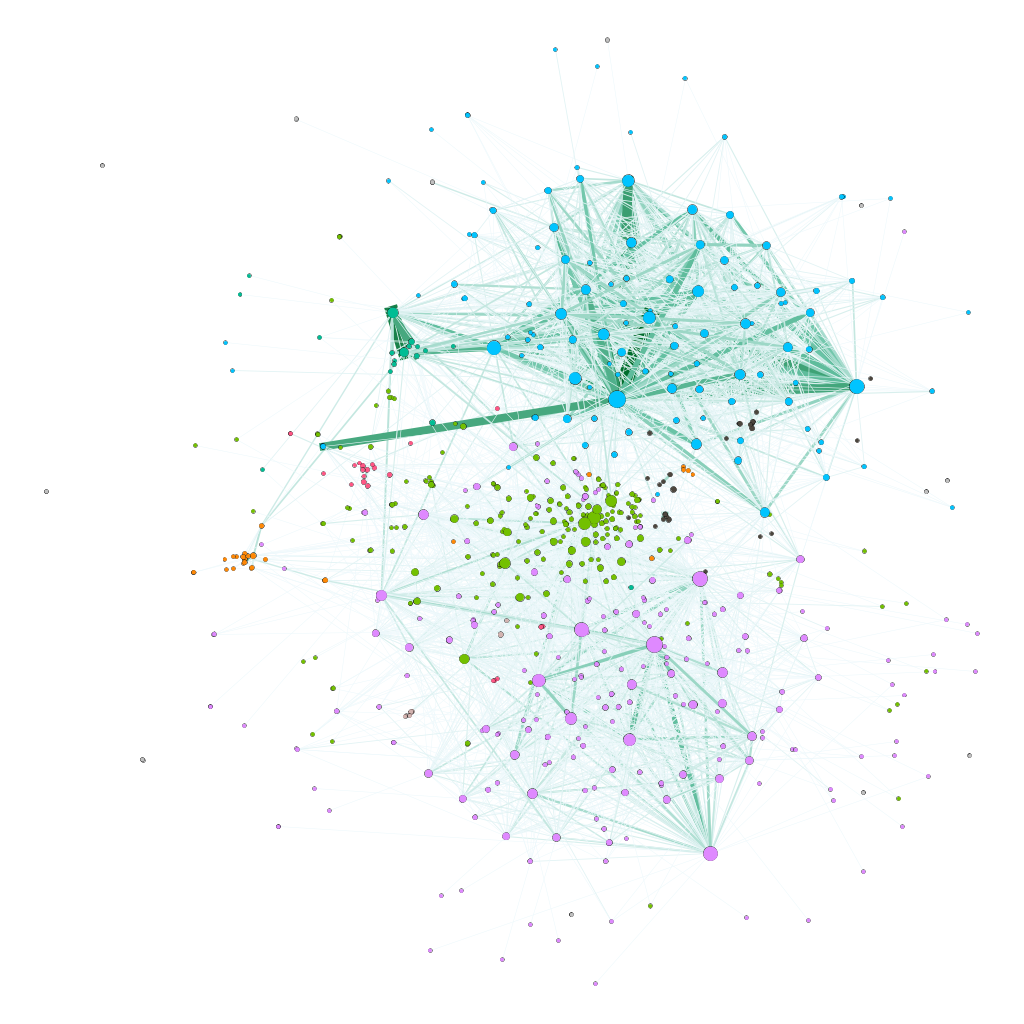
\includegraphics[width=0.6\linewidth]{dec2016net.png}
B.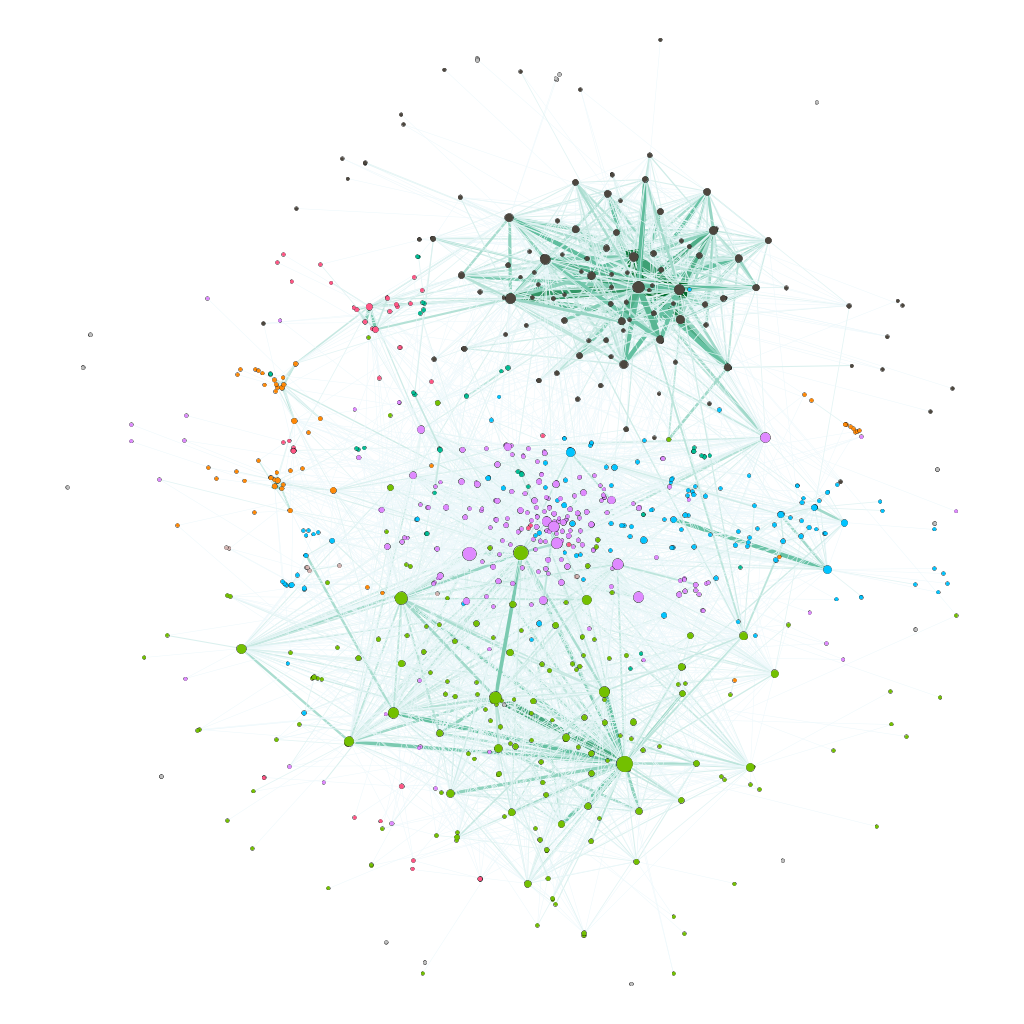
\includegraphics[width=0.6\linewidth]{jan2017net.png}
\caption{\textbf{Networks of user interactions before the ban} Gephi visualization of networks of users who had posted within the subreddit r/altright in January 2017. Edges exist between two users if they posted in at least two threads together. Edges are weighted by the total number of threads the users mutually posted in. Nodes are colored by their modularity class, and edges are colored by their weight. A. December 2016. The blue community comments approximately on r/debatealtright. The green community corresponds with popular subreddits, and the purple community corresponds with popular subreddits including r/The\textunderscore Donald. The orange community on the far left corresponds with r/MGOTW (Men Going Their Own Way) and r/theredpill. B. January 2017. Communities here are very similar to those in Fig. \ref{fig:1}A, with similar visual correspondences.}
\label{fig:1}
\end{figure}


\begin{figure}
\centering
A.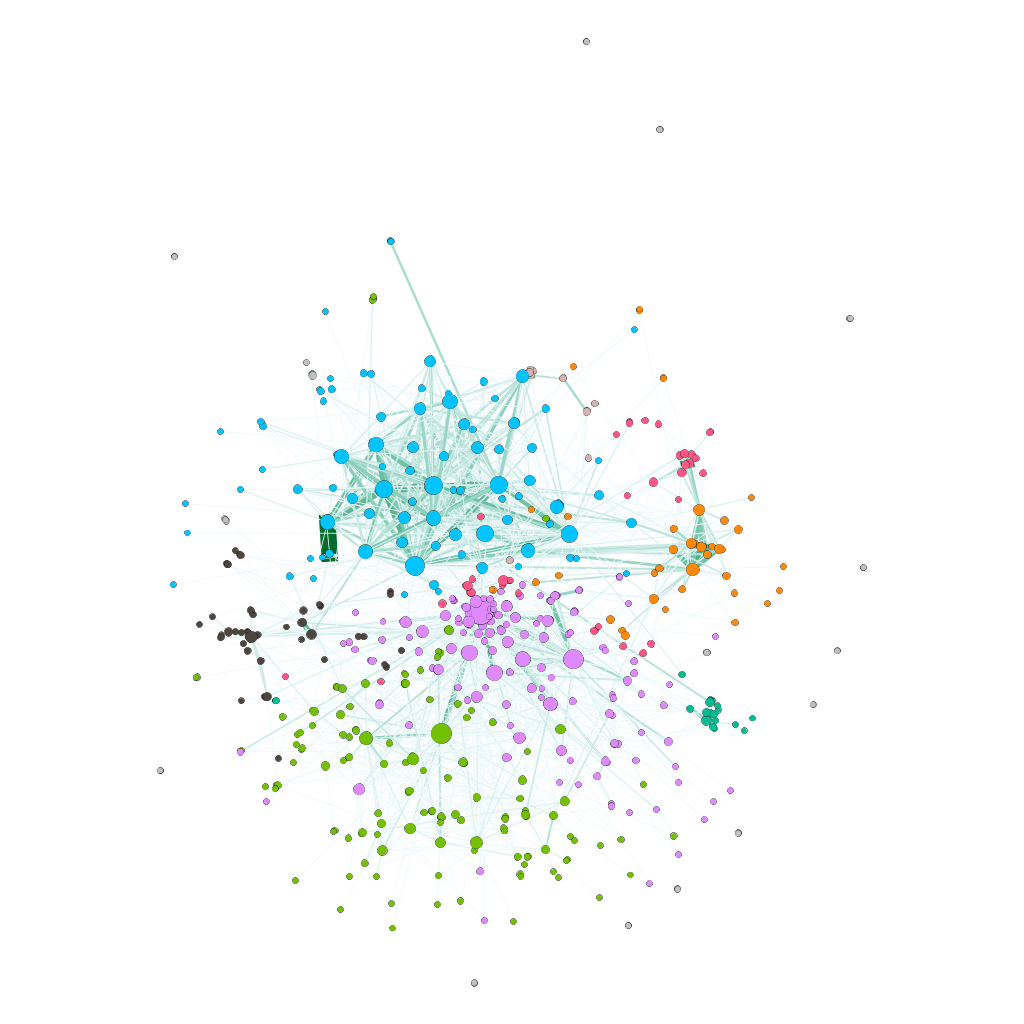
\includegraphics[width=0.6\linewidth]{feb2017net.png} 
B.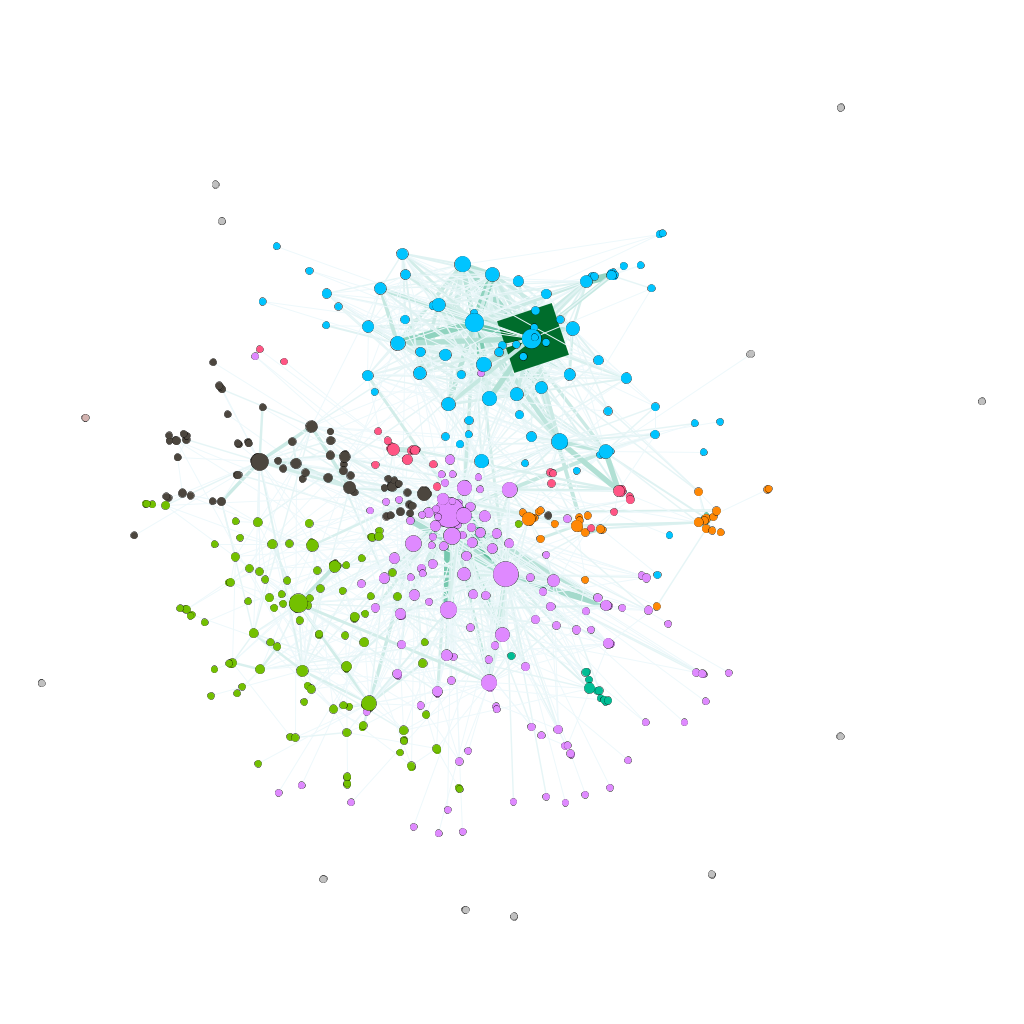
\includegraphics[width=0.6\linewidth]{mar2017netbad.png}
\caption{\textbf{Networks of user interactions after the ban} Similar Gephi visualizations of networks as Fig. \ref{fig:1}. Edges exist between two users if they posted in at least two threads together. Edges are weighted by the total number of threads the users mutually posted in. Nodes are colored by their modularity class, and edges are colored by their weight. A. February 2017. A noticeable reduction in the absolute number of qualified members is clear. However, the communities are similar to those prior to the ban. The highly connected blue community corresponds approximately with r/debatealtright. The purple and green communities correspond with popular subreddits or including r/The\textunderscore Donald. B. March 2017. There is an erroneous edge (green square) that is significantly greater in weight than any other edge in the network. The same community structure appears to persist from previous months.}
\label{fig:2}
\end{figure}


\begin{table}[]
\centering
\caption{The number of nodes and number of edges are recorded for each of the networks created for each month.}
\label{table1}
\begin{tabular}{lll}
                                   & Number of Nodes          & Number of Edges           \\ \cline{2-3} 
\multicolumn{1}{l|}{December 2016} & \multicolumn{1}{l|}{729} & \multicolumn{1}{l|}{3972} \\ \cline{2-3} 
\multicolumn{1}{l|}{January 2017}  & \multicolumn{1}{l|}{836} & \multicolumn{1}{l|}{4228} \\ \cline{2-3} 
\multicolumn{1}{l|}{February 2017} & \multicolumn{1}{l|}{570} & \multicolumn{1}{l|}{1875} \\ \cline{2-3} 
\multicolumn{1}{l|}{March 2017}    & \multicolumn{1}{l|}{497} & \multicolumn{1}{l|}{1590} \\ \cline{2-3} 
\end{tabular}
\end{table}


\begin{table}[]
\centering
\caption{Below shows the table for each of the metrics measured in the null model and real networks. Mean ($\mu$) and real values are in units corresponding with the network metric. }
\label{table2}
\begin{tabular}{lllll}
                                                 & Null $\mu$                     & Real                        & $z$                          & $p$                                      \\ \cline{2-5} 
\multicolumn{1}{l|}{Mean degree}                 & \multicolumn{1}{l|}{6.91}  & \multicolumn{1}{l|}{6.58}   & \multicolumn{1}{l|}{-0.63} & \multicolumn{1}{l|}{0.53}              \\ \cline{2-5} 
\multicolumn{1}{l|}{Diameter}                    & \multicolumn{1}{l|}{9.01}  & \multicolumn{1}{l|}{8}      & \multicolumn{1}{l|}{-1.01} & \multicolumn{1}{l|}{0.31}              \\ \cline{2-5} 
\multicolumn{1}{l|}{Mean shortest path length}   & \multicolumn{1}{l|}{7.56}  & \multicolumn{1}{l|}{8.17}   & \multicolumn{1}{l|}{3.26}  & \multicolumn{1}{l|}{\textbf{0.001}}    \\ \cline{2-5} 
\multicolumn{1}{l|}{Assortativity}               & \multicolumn{1}{l|}{-0.11} & \multicolumn{1}{l|}{0.0046} & \multicolumn{1}{l|}{3.01}  & \multicolumn{1}{l|}{\textbf{0.003}}    \\ \cline{2-5} 
\multicolumn{1}{l|}{Density}                     & \multicolumn{1}{l|}{0.012} & \multicolumn{1}{l|}{0.012}  & \multicolumn{1}{l|}{-0.63} & \multicolumn{1}{l|}{0.53}              \\ \cline{2-5} 
\multicolumn{1}{l|}{Mean clustering coefficient} & \multicolumn{1}{l|}{0.26}  & \multicolumn{1}{l|}{0.23}   & \multicolumn{1}{l|}{-1.61} & \multicolumn{1}{l|}{0.11}              \\ \cline{2-5} 
\multicolumn{1}{l|}{Number of cliques}           & \multicolumn{1}{l|}{1171}  & \multicolumn{1}{l|}{1051}   & \multicolumn{1}{l|}{-1.32} & \multicolumn{1}{l|}{0.19}              \\ \cline{2-5} 
\multicolumn{1}{l|}{Transitivity}                & \multicolumn{1}{l|}{0.24}  & \multicolumn{1}{l|}{0.27}   & \multicolumn{1}{l|}{2.03}  & \multicolumn{1}{l|}{0.04}              \\ \cline{2-5} 
\multicolumn{1}{l|}{Community overlay distance}  & \multicolumn{1}{l|}{11.03} & \multicolumn{1}{l|}{20.53}  & \multicolumn{1}{l|}{7.51}  & \multicolumn{1}{l|}{\textbf{$5.83*10^{-14}$}} \\ \cline{2-5} 
\end{tabular}
\end{table}

\end{document}
